%%%%%%%%%%%%%%%%%%%%%%%%%%%%%%%%%%%%%%%%%
% Journal Article
% LaTeX Template
% Version 1.4 (15/5/16)
%
% This template has been downloaded from:
% http://www.LaTeXTemplates.com
%
% Original author:
% Frits Wenneker (http://www.howtotex.com) with extensive modifications by
% Vel (vel@LaTeXTemplates.com)
%
% License:
% CC BY-NC-SA 3.0 (http://creativecommons.org/licenses/by-nc-sa/3.0/)
%
%%%%%%%%%%%%%%%%%%%%%%%%%%%%%%%%%%%%%%%%%

%----------------------------------------------------------------------------------------
%	PACKAGES AND OTHER DOCUMENT CONFIGURATIONS
%----------------------------------------------------------------------------------------

\documentclass[twoside,twocolumn]{article}

\usepackage{blindtext} % Package to generate dummy text throughout this template 

\usepackage{url}
\usepackage{hyperref} 

\usepackage[sc]{mathpazo} % Use the Palatino font
\usepackage[T1]{fontenc} % Use 8-bit encoding that has 256 glyphs
\linespread{1.05} % Line spacing - Palatino needs more space between lines
\usepackage{microtype} % Slightly tweak font spacing for aesthetics

\usepackage{biblatex}
\addbibresource{cs385.bib}

\usepackage[english]{babel} % Language hyphenation and typographical rules

\usepackage[hmarginratio=1:1,top=32mm,columnsep=20pt]{geometry} % Document margins
\usepackage[hang, small,labelfont=bf,up,textfont=it,up]{caption} % Custom captions under/above floats in tables or figures
\usepackage{booktabs} % Horizontal rules in tables

\usepackage{lettrine} % The lettrine is the first enlarged letter at the beginning of the text

\usepackage{graphicx}
\graphicspath{ {./} }

\usepackage{lipsum}
\usepackage{enumitem} % Customized lists
\setlist[itemize]{noitemsep} % Make itemize lists more compact

\usepackage[utf8]{inputenc}

\usepackage{xcolor}   % For coloring text 
\usepackage{listings} % For code snippets 
\lstdefinelanguage
   [x64]{Assembler}     % add a "x64" dialect of Assembler
   [x86masm]{Assembler} % based on the "x86masm" dialect
   % with these extra keywords:
   {morekeywords={CDQE,CQO,CMPSQ,CMPXCHG16B,JRCXZ,LODSQ,MOVSXD, %
                  POPFQ,PUSHFQ,SCASQ,STOSQ,IRETQ,RDTSCP,SWAPGS, %
                  rax,rdx,rcx,rbx,rsi,rdi,rsp,rbp, %
                  r8,r8d,r8w,r8b,r9,r9d,r9w,r9b}} % etc.

\usepackage{abstract} % Allows abstract customization
\renewcommand{\abstractnamefont}{\normalfont\bfseries} % Set the "Abstract" text to bold
\renewcommand{\abstracttextfont}{\normalfont\small\itshape} % Set the abstract itself to small italic text

\usepackage{titlesec} % Allows customization of titles
\renewcommand\thesection{\Roman{section}} % Roman numerals for the sections
\renewcommand\thesubsection{\roman{subsection}} % roman numerals for subsections
\titleformat{\section}[block]{\large\scshape\centering}{\thesection.}{1em}{} % Change the look of the section titles
\titleformat{\subsection}[block]{\large}{\thesubsection.}{1em}{} % Change the look of the section titles

\usepackage{fancyhdr} % Headers and footers
\pagestyle{fancy} % All pages have headers and footers
\fancyhead{} % Blank out the default header
\fancyfoot{} % Blank out the default footer
\fancyhead[C]{Tweet Popularity and Follower Count $\bullet$ December 2021 $\bullet$ Final Project} % Custom header text
\fancyfoot[RO,LE]{\thepage} % Custom footer text

\usepackage{titling} % Customizing the title section

\usepackage{hyperref} % For hyper-links in the PDF

\usepackage{array} %for arrays in tables

\usepackage{float} %for non floating figures

%----------------------------------------------------------------------------------------
%	TITLE SECTION
%----------------------------------------------------------------------------------------

\setlength{\droptitle}{-4\baselineskip} % Move the title up

%\pretitle{\begin{center}\Huge\bfseries % Article title formatting
%\posttitle \end{center}} % Article title closing formatting
\title{Tweet Popularity and Follower Count \\ CS 485 Final Project} % Article title

\author{% ends 
  \textsc{Temi Kelly} \\[1ex] % Your name
  \normalsize Emory University \\ % Your institution
  \normalsize \href{mailto:agkell3@emory.edu}{agkell3@emory.edu} % Your email address
  \and % Uncomment if 2 authors are required, duplicate these 4 lines if more
  \textsc{Fiona Lau} \\[1ex] % Second author's name
  \normalsize Emory University \\ % Second author's institution
  \normalsize \href{mailto:fhlau@emory.edu}{fhlau@emory.edu} % Second author's email address
  \and % Uncomment if 2 authors are required, duplicate these 4 lines if more
} % end of \author 

\date{December 9, 2021} % Leave empty to omit a date
\renewcommand{\maketitlehookd}{%+

%##########  ABSTRACT GOES HERE ############################%
\begin{abstract}
  
  %{\color{blue}
  %  Here you put a brief description of what this project is all about, what you did and what your results show. 
  %  The goal is to make the reader interested in reading the rest of the report, often s tarting with your conclusions / discussion.
  %  Keep this in mind when you write the discussion section. 
  %}
  
\noindent Twitter has become a major source of information spread, with 206 million daily active users worldwide \cite{1}. Examining the impact that a viral tweet has on an individual user gives insight into predicting how information disseminates and whose content becomes popular. We wish to further explore the relationship between twitter user popularity and tweet virality. More specifically, we want to examine the importance of follower count. In investigating this, we will explore the potential “rich get richer” phenomenon as applied to tweets. We want to show that the rate of increase in followers in the wake of a viral tweet is related to the amount of followers before the tweet. Using statistical inference, we did not find a significant increase in follower rates after a viral tweet compared to before the tweet.

  %The project Malloc-lab was focused on how your computer handles memory management inside virtual memory.
\end{abstract}
}

%----------------------------------------------------------------------------------------

\begin{document}

% Print the title
\maketitle

%----------------------------------------------------------------------------------------
%	ARTICLE CONTENTS
%----------------------------------------------------------------------------------------

\section{Introduction}
We analyze the impact of virality of a tweet on an individual by comparing Twitter users’ follower count in the time before and after a viral tweet they made. We define each user’s “viral tweet” to be their tweet with the largest number of retweets - or number of users reposting their tweet. We want to explore how the number of followers gained from a viral tweet relates to the number of followers users had previously. In particular, we ask how does the follower growth rate after a viral tweet compare with the follower growth rate before? Does this rate vary depending on the number of followers?\\

There is minimal research studying the network influence of users on social media across the entire time duration that they are active on a platform. This is likely due to the difficulties with historical data collection and the complex nature of social media interactions varying from platform to platform and over time with application updates. Much research into social media has focused on understanding the impact of a viral post on trending topics, rather than understanding the impact on the user \cite{9}\cite{10}\cite{11}. Predicting the virality of a single tweet or a group of tweets has been explored in depth both with regards to user popularity \cite{2} and with regards to information spreading \cite{3}. Similar studies have been done on other platforms, such as predicting video view counts on Youtube \cite{4} or likes on an Instagram photo \cite{5}. This research fails to examine the importance of the individual user as the information spreader and does not analyze the individual users’ popularity over the entire course of their careers.\\

Understanding the effect of tweet popularity on the user’s following base is novel compared to previous problems like predicting tweet virality or even measuring the impact of a viral tweet on a hashtag. This is because we focus on virality in the context of an individual users’ retweet and follower history. Rather than predicting virality, which many of the studies in our Related Works section focus on, we will be looking at the impact of virality on an individual’s follower rate.\\

Our analysis utilizes a large Twitter dataset with users tweet and follower histories over the course of nearly 10 years. The data comes from the paper, “The Evolution of Retweet Rates” which examined the timeline of a twitter user’s retweet rate per follower over the course of their careers \cite{6}. The study shows a relationship between followers and retweet count and examines user’s impact on the individual level. However, it fails to understand the relationship between followers and retweet count trajectories in relation to the user’s viral tweets. We use this study’s dataset containing userid’s and historical tweets, retweet counts, and follower counts for each user. We want to use this time series data to explore the co-dependent relationship between follower count and retweet count. We plan on examining the average natural follower growth pattern over time for all users and using this as a baseline to track follower growth over different time spans following a “viral” tweet.

\section{Related Work}

%\lettrine[nindent=0em,lines=3]{W}

% PLEASE remove this text from the final report, you can simply comment it out with '%'
% {\color{blue} \emph  
% The focus of your writing for this report should be the Dynamic Memory Allocation (chapter 9.9 in Bryant \& O'halloran). 
% In the introduction you must introduce the topic of dynamic memory allocation (WHAT) and motivate the need for it (WHY).
% You will need to explain the challenges and mention solutions that have been proposed (implicit lists, explicit list, etc.).
% You will briefly mention what system you have chosen to implement and and why.

% (Hint: Try to connect the text nicely between sections. 
% Also, typically, you would end the introduction by describing the rest of the paper)
% }

Much of the related work in this field focuses specifically on predicting the final number of retweets of an original tweet. There are many existing methods to model the popularity of tweets, including epidemic based models, complex machine learning methods, and more probabilistic focused models. Often, the models need to observe the tweet and its retweets for some time, varying from 5 minutes to 1 hour, before they are able to make a final tweet count prediction using factors such as the number of followers, the depth of the retweet in a retweet graph, and how many retweets there were in that observation period.  \\ \\
Many of these recent methods are similar to the epidemic SIR, SIS and SEIZ models that we have discussed in class and use parameters like the “infectiousness” of a tweet. In the recent SEISMIC model, the infectiousness encompasses the observed history of retweets to measure a probabilistic likelihood of future reshares. This metric is then used to predict the ultimate total number of reshares, or the cascade size of a tweet \cite{7}. In this case, the infectiousness parameter is allowed to vary over time, representing the more realistic nature of information cascades and importance of non-constant time series data in predicting future retweets.\\

Other retweet prediction models focus more on probabilistic methods, such as a Bayesian probabilistic approach that uses summary graphs of the followers of the user, the number of retweets of other tweets and the amount of early retweet times \cite{2}. Another early probabilistic collaborative filtering method takes a different approach, using retweet patterns from the tweet source, a retweeter, and the tweet content to learn the correlation between users and topics in order to predict users preference for that topic \cite{3}.\\
 
 As time has gone on and social media platforms have been updated, many models for predicting tweet virality are antiquated. The models are based around the old structure for retweets, which included the retweeter creating a new tweet that starts with “RT @”, followed by the username of the original tweeter or most recent retweeter, and then the content of the post. When a long chain of retweeting occurred, the tweet content would become muddled with unnecessary information about the retweet. Since the structural change in retweeting, we believe that it is very likely that the number of retweets, on average, has increased due to the updated aesthetics.\\
 
 In addition, many models in this field fail to take into account characteristics of tweets that we believe impact the potential retweets. For example, the time of day of the tweet, the content of the tweet and current trending topics. Furthermore, most models make an assumption of conditional independence between followers, meaning that they assume two people who have retweeted the same tweet do not follow each other. We believe this is a major oversight, aligned with not taking tweet content into account, that would lead to poor predictability performance for most of these models on data sets that are from more niche groups within twitter, such as a fandom.\\
 
There are a lot of topics left to be explored and further developed currently. For example, the SEISMIC and Bayesian papers leave room for improvement by excluding the posted time of day of a tweet from their models. The times of the day when users are most active on Twitter and whether or not a tweet was posted in these time periods may influence how likely the post will be reshared. Is time of day alone a strong enough factor in determining whether or not a tweet can reach virality? Furthermore, other questions that are interesting include: 
 
\begin{itemize}
  \item \textit{Can we predict virality of a tweet given the content of the tweet and an observed list of topics of interest for followers? } This could be pursued by developing a model that can crawl a twitter user’s page to find general topics that they are interested in based on their tweet and retweet history. Then, one could examine the likelihood for individual users to retweet a tweet if it is about one of their topics of interest and it is posted by a user they follow. This likelihood can then be implemented into a potential model’s prediction algorithm.\\
  \item \textit{How does the number of people that you follow that have retweeted the same tweet impact your likelihood of retweeting it?} This would require building a network of twitter users who are followers of each other and then examining the retweet network that is used in many of these models.\\
  \item \textit{How does the “rich get richer” phenomenon relating to users with high follower counts and their resulting viral tweets play out in real observed data?} This could be explored by looking at time series data depicting user follower count and viral retweet count over time. Much of the research so far focuses on using follower count as a parameter to predict number of retweets, but we are more interested in exploring a feedback loop relationship between follower gain and tweet virality. A deeper understanding of this complex relationship may help us improve upon current tweet popularity prediction algorithms. We are most interested in examining this particular research question. 

\end{itemize}
In the rest of this paper, we will explore this complex relationship in an attempt to gain a deeper understanding of how follower count is impacted by viral tweets. We will begin with an explanation of our dataset and methods for our statistical inference. Then, we will quantify our results and explore what are the next steps in this line of research.

\section{Data}
As stated earlier, much of the research related to Twitter has been focused on using different static tweet related features to predict virality. As a result, procuring a time series dataset with all tweets for each user as well as their historical follower counts, dates of tweeting, and retweet counts was a difficult task. \\

We found a dataset that contains tweets over the course of nearly 10 years from the study “The Evolution of Retweet Rates in Twitter User Careers” \cite{6}. This dataset includes twitter information for users who retweeted a U.S. Presidential or vice-presidential candidate five or more times between 2009 and 2018. These 69 million tweets encompass 23,000 users, containing every single original tweet from the users, but excludes any retweets from their profile. To determine the number of followers each user had over the course of their twitter careers, the researchers performed a crawl of each user’s number of followers at different time intervals using the Internet Archive’s Wayback Machine. Each of the 69 million tweets is accompanied by the timestamp of the tweet, a count of its number of retweets up to June 2018, the other users who retweeted it, and an estimate of the user’s follower count at the time of the tweet if an exact count was not available. 

\section{Methods}
Due to this dataset being 69 million records, we needed to heavily clean the data before we were able to easily open and analyze it. We began by removing tweets with only 1 or 0 retweets to reduce the data size complexity. We thought that these tweets would be irrelevant for our analysis because it is unlikely that tweets with so few retweets exposed the user to new followers. This reduced our dataset to 15 million records. In our virality analysis, we also discarded users who did not have at least one viral tweet, which we define as reaching a total of 500 or more retweets. We identified the user’s most viral tweet as their tweet with the highest number of total retweets out of all tweets they made in their career. The remainder of our study focuses on the relationship between each user’s most viral tweet and the rate of change in followers before and after the user made the viral tweet.

\begin{figure}[H]
\begin{tabular}{ | m{5em} | m{2cm}| m{1.5cm} | } 
  \hline
    & Mean & Median \\ 
  \hline
  Number of Total Tweets & 507 & 255 \\ 
  \hline
  Average Number of Retweets & 58,041,697,507 & 5 \\ 
  \hline
  Average Number of Followers & 11,470 & 7,631 \\ 
  \hline
\end{tabular}\\
\caption{Preliminary Analysis of Tweet, Retweet, and Follower Counts}
\end{figure}

We begin by performing some preliminary analysis of the data. We compute each user’s total number of tweets, average number of retweets, and average number of followers and we display the means and medians in Figure 1. In Figure 2 and Figure 3, we see that the frequencies of the total number of tweets users make across their career follows a power law. We also see that users have an average follower count of 11,470, but the follower distribution has a heavy tail with larger values (Figure 4). \\



\begin{figure}[h]
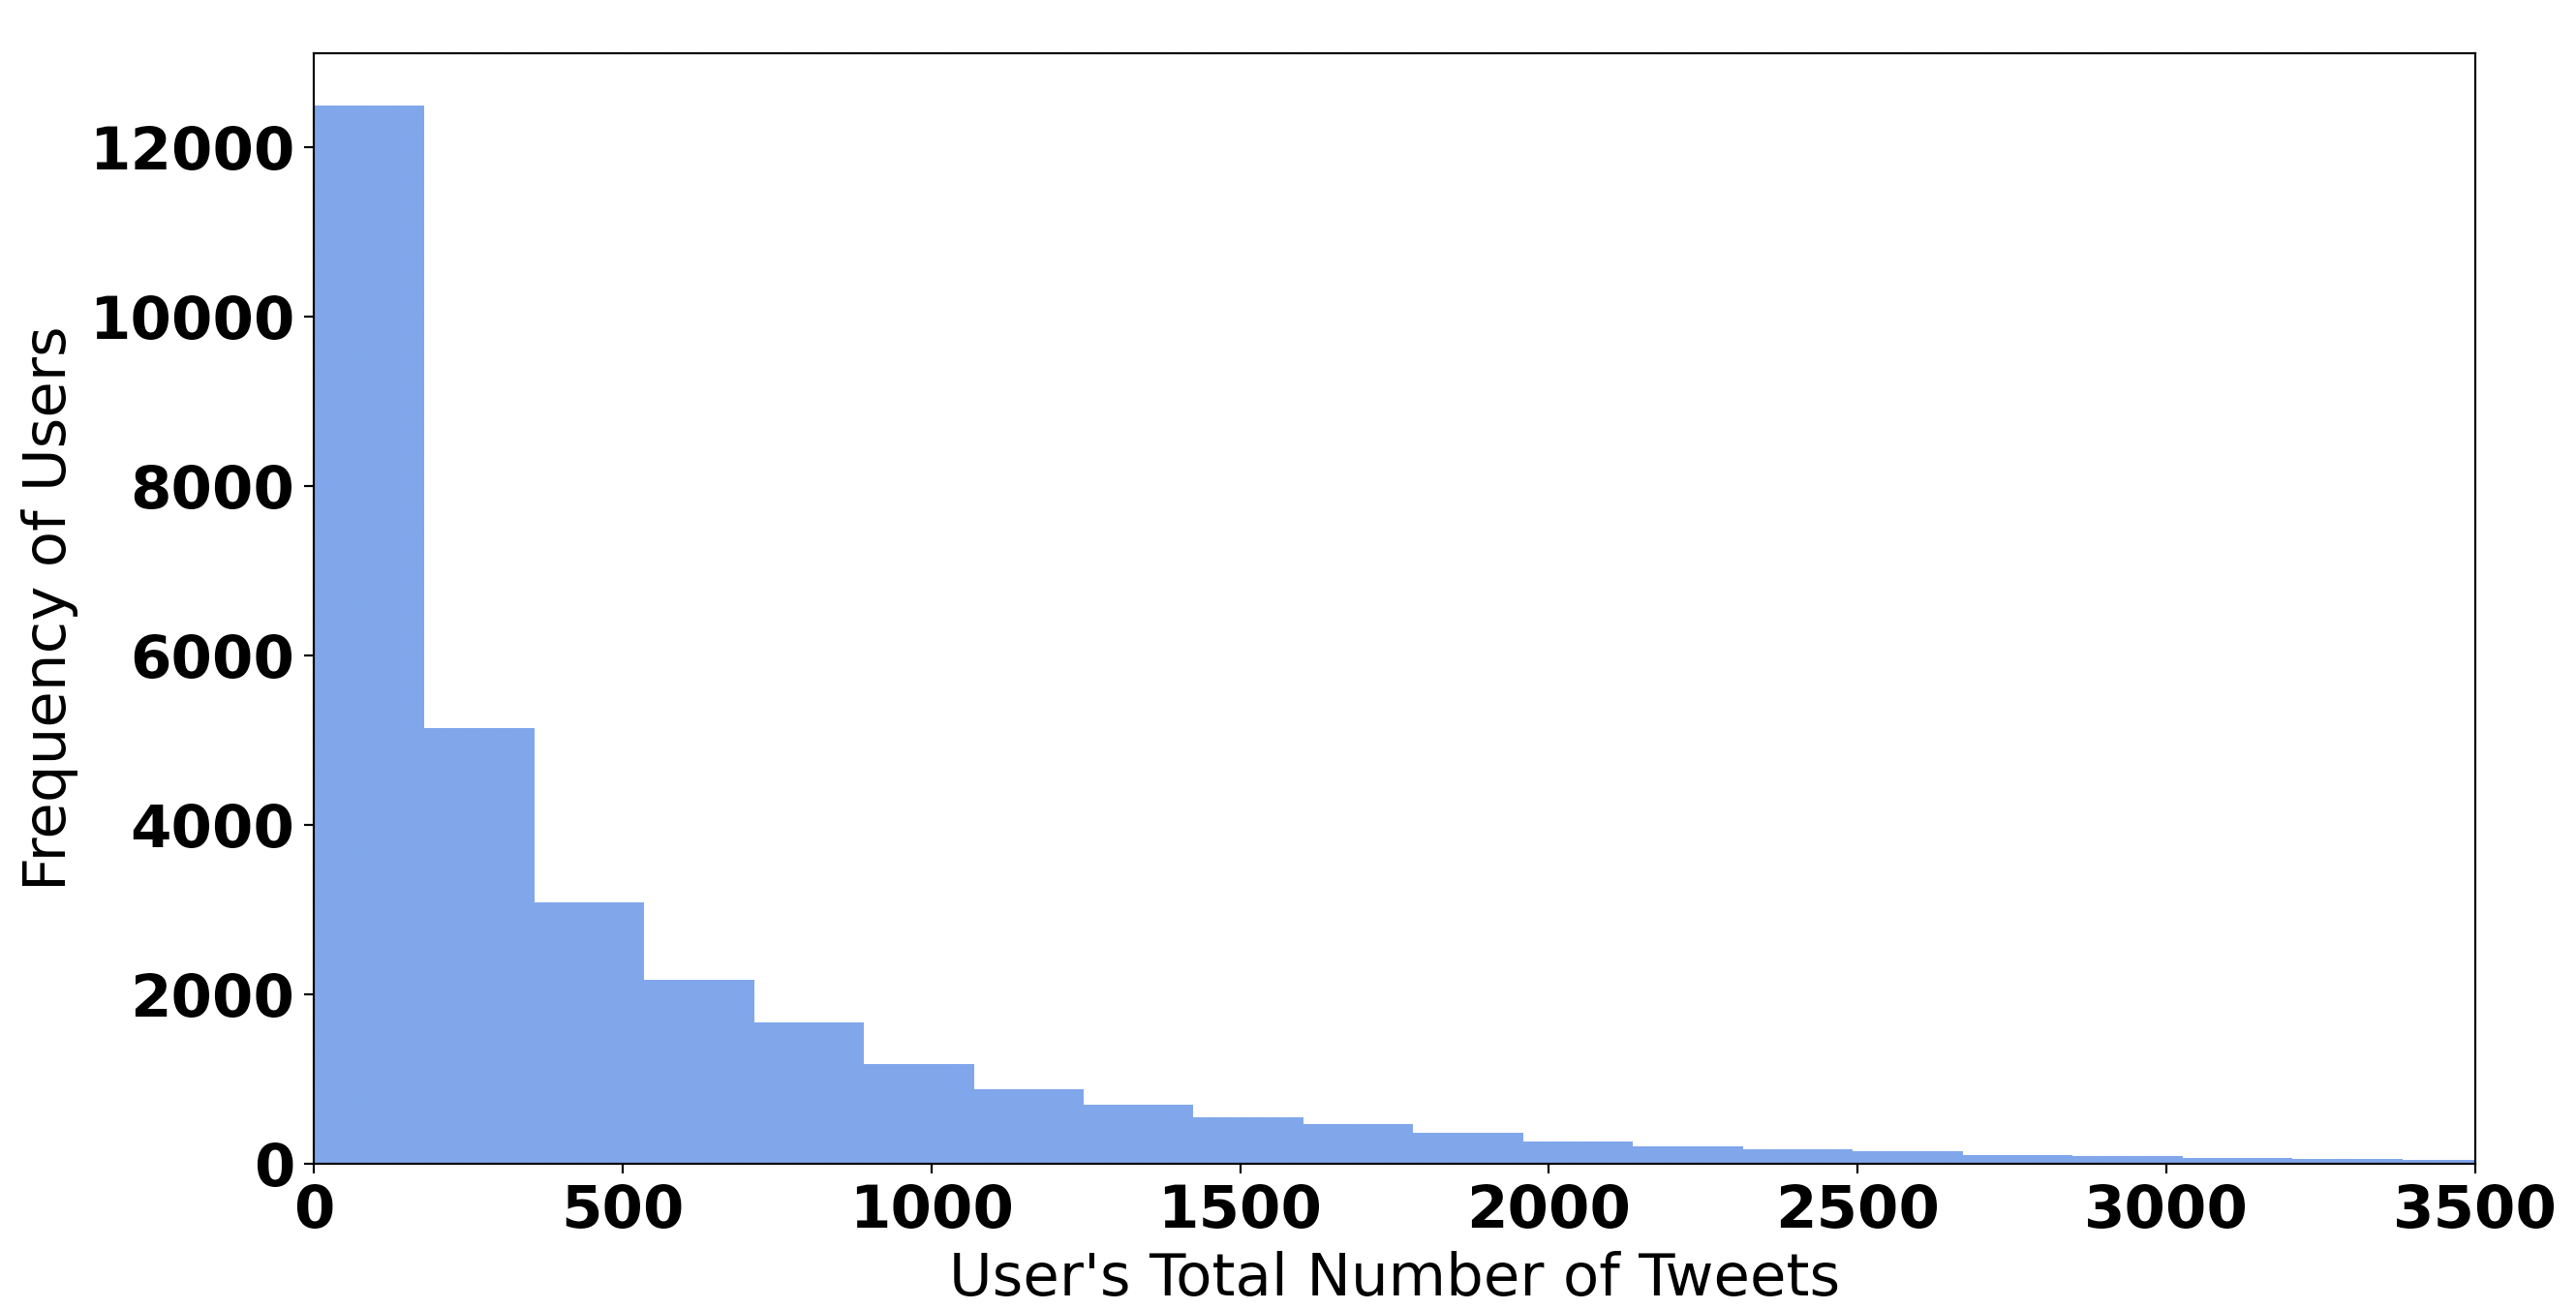
\includegraphics[width=7cm]{p1.png}
\caption{Histogram of User's Total Number of Tweets Over Entire Twitter Career}
\end{figure}

\begin{figure}[h]
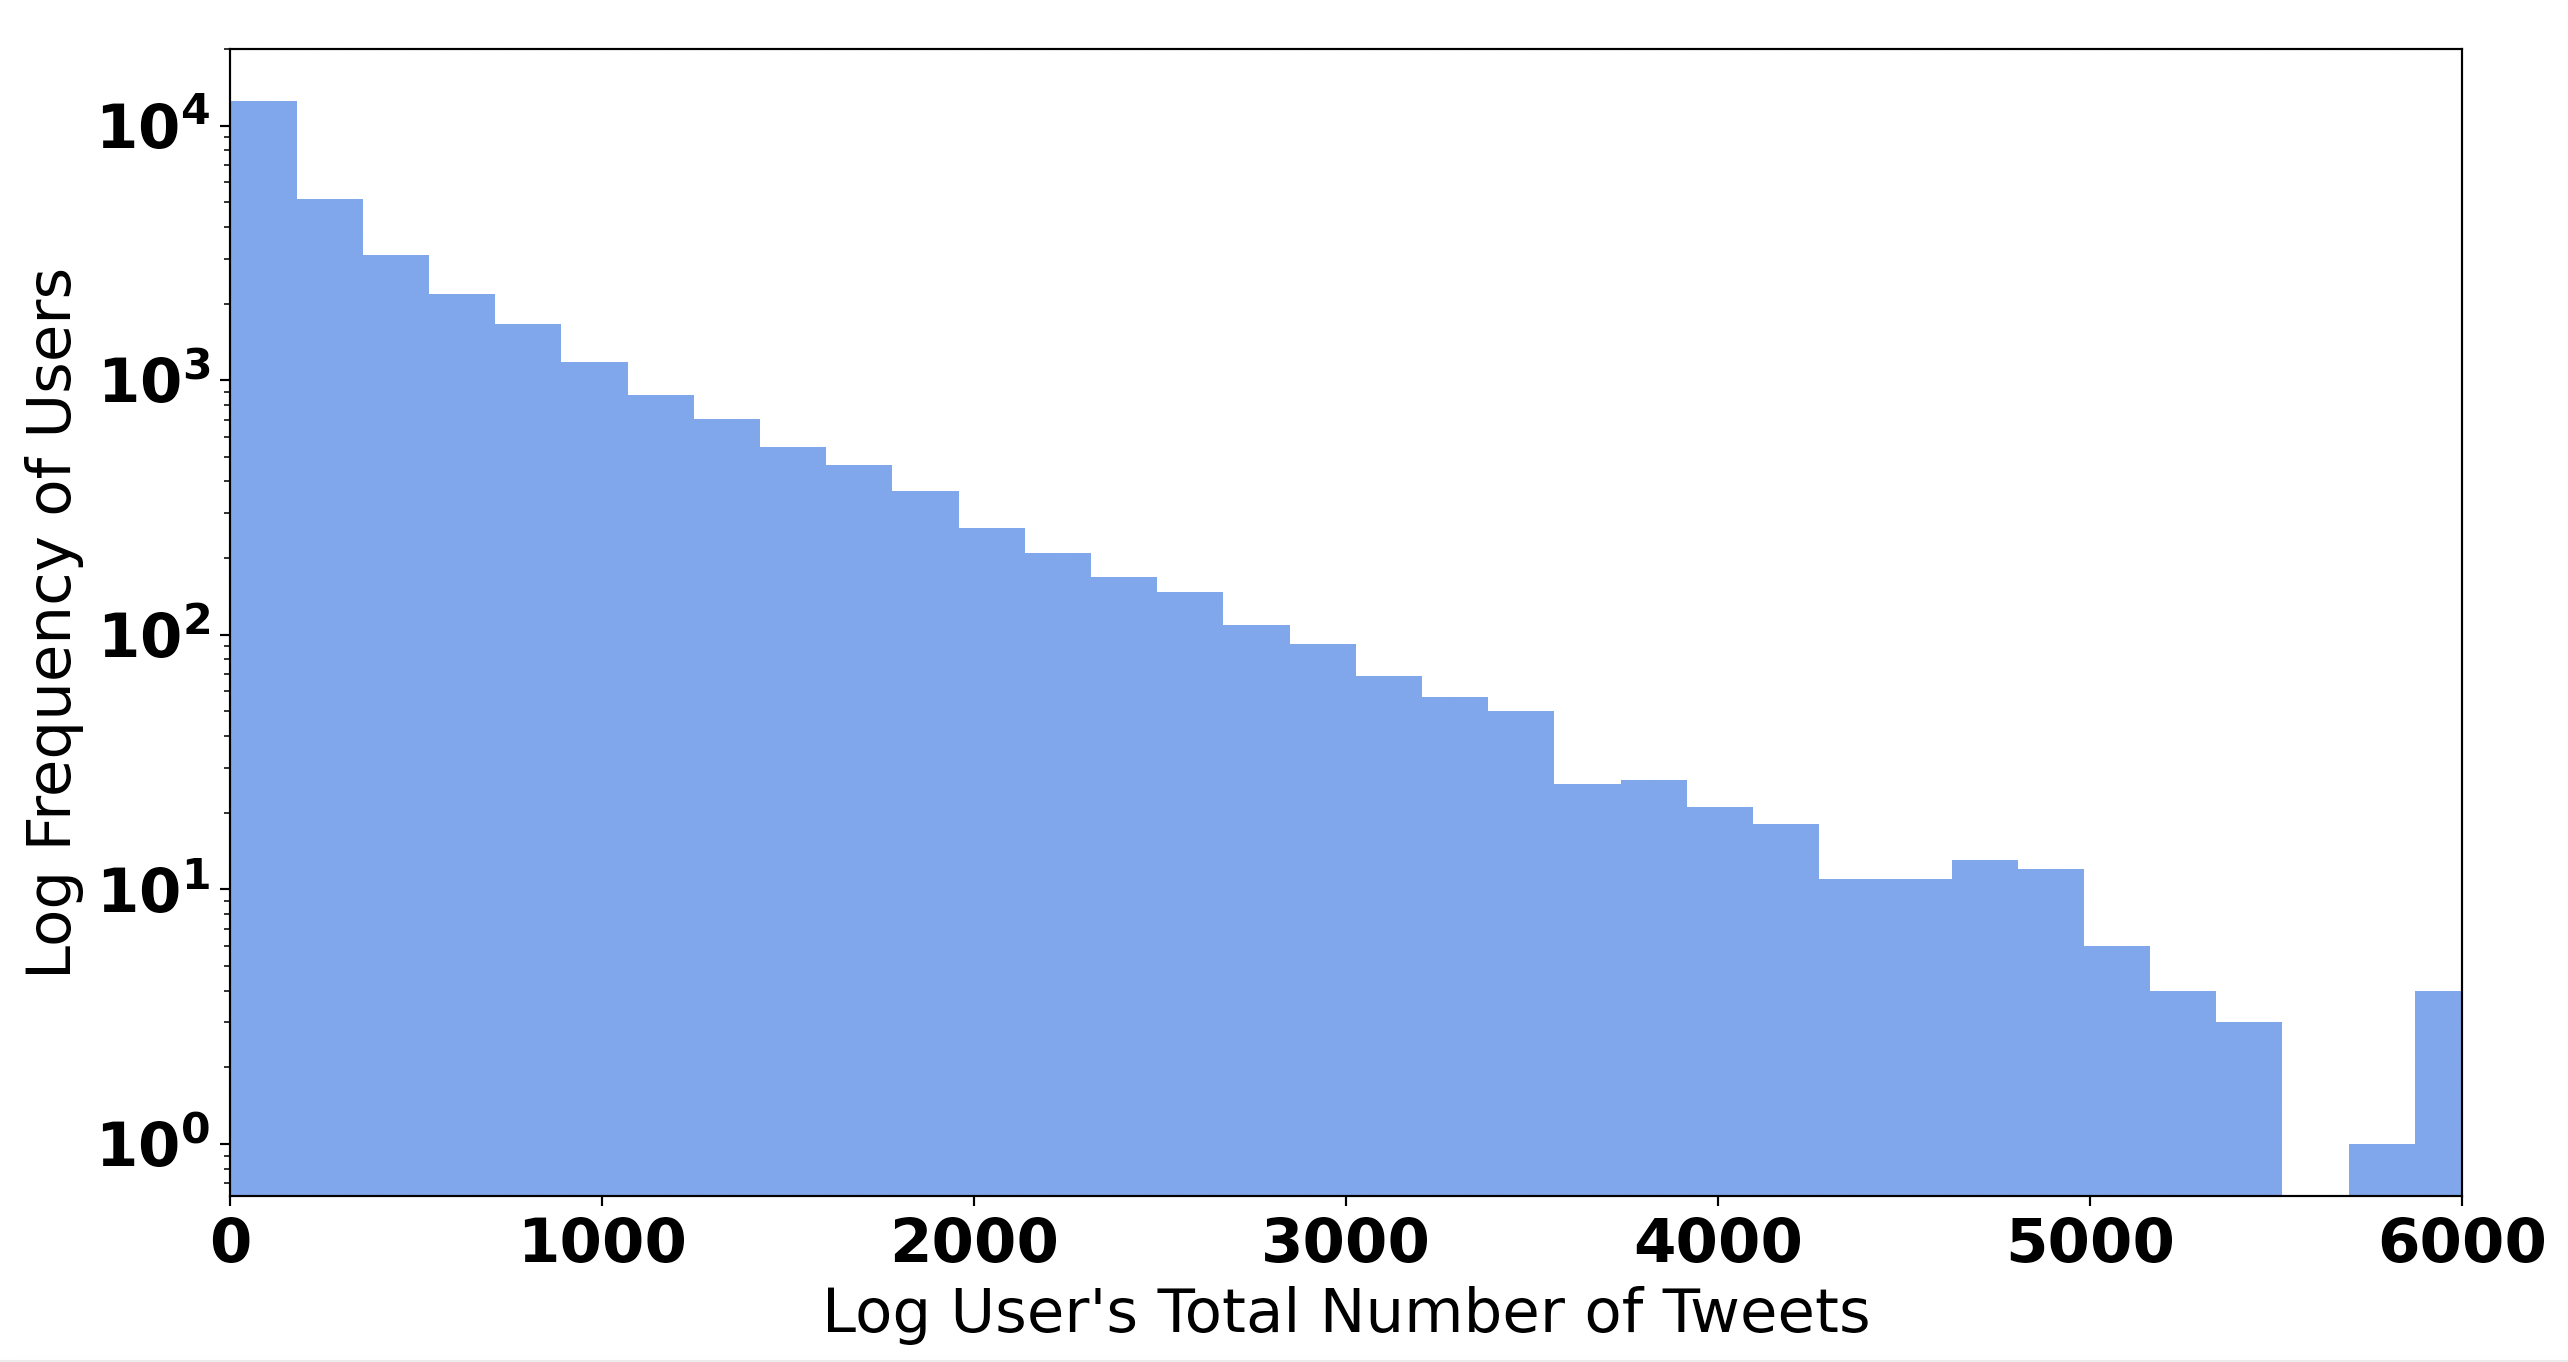
\includegraphics[width=7.5cm]{p2.png}
\caption{Log-Log Histogram of User's Total Number of Tweets Over Entire Twitter Career}
\end{figure}

\begin{figure}[h]
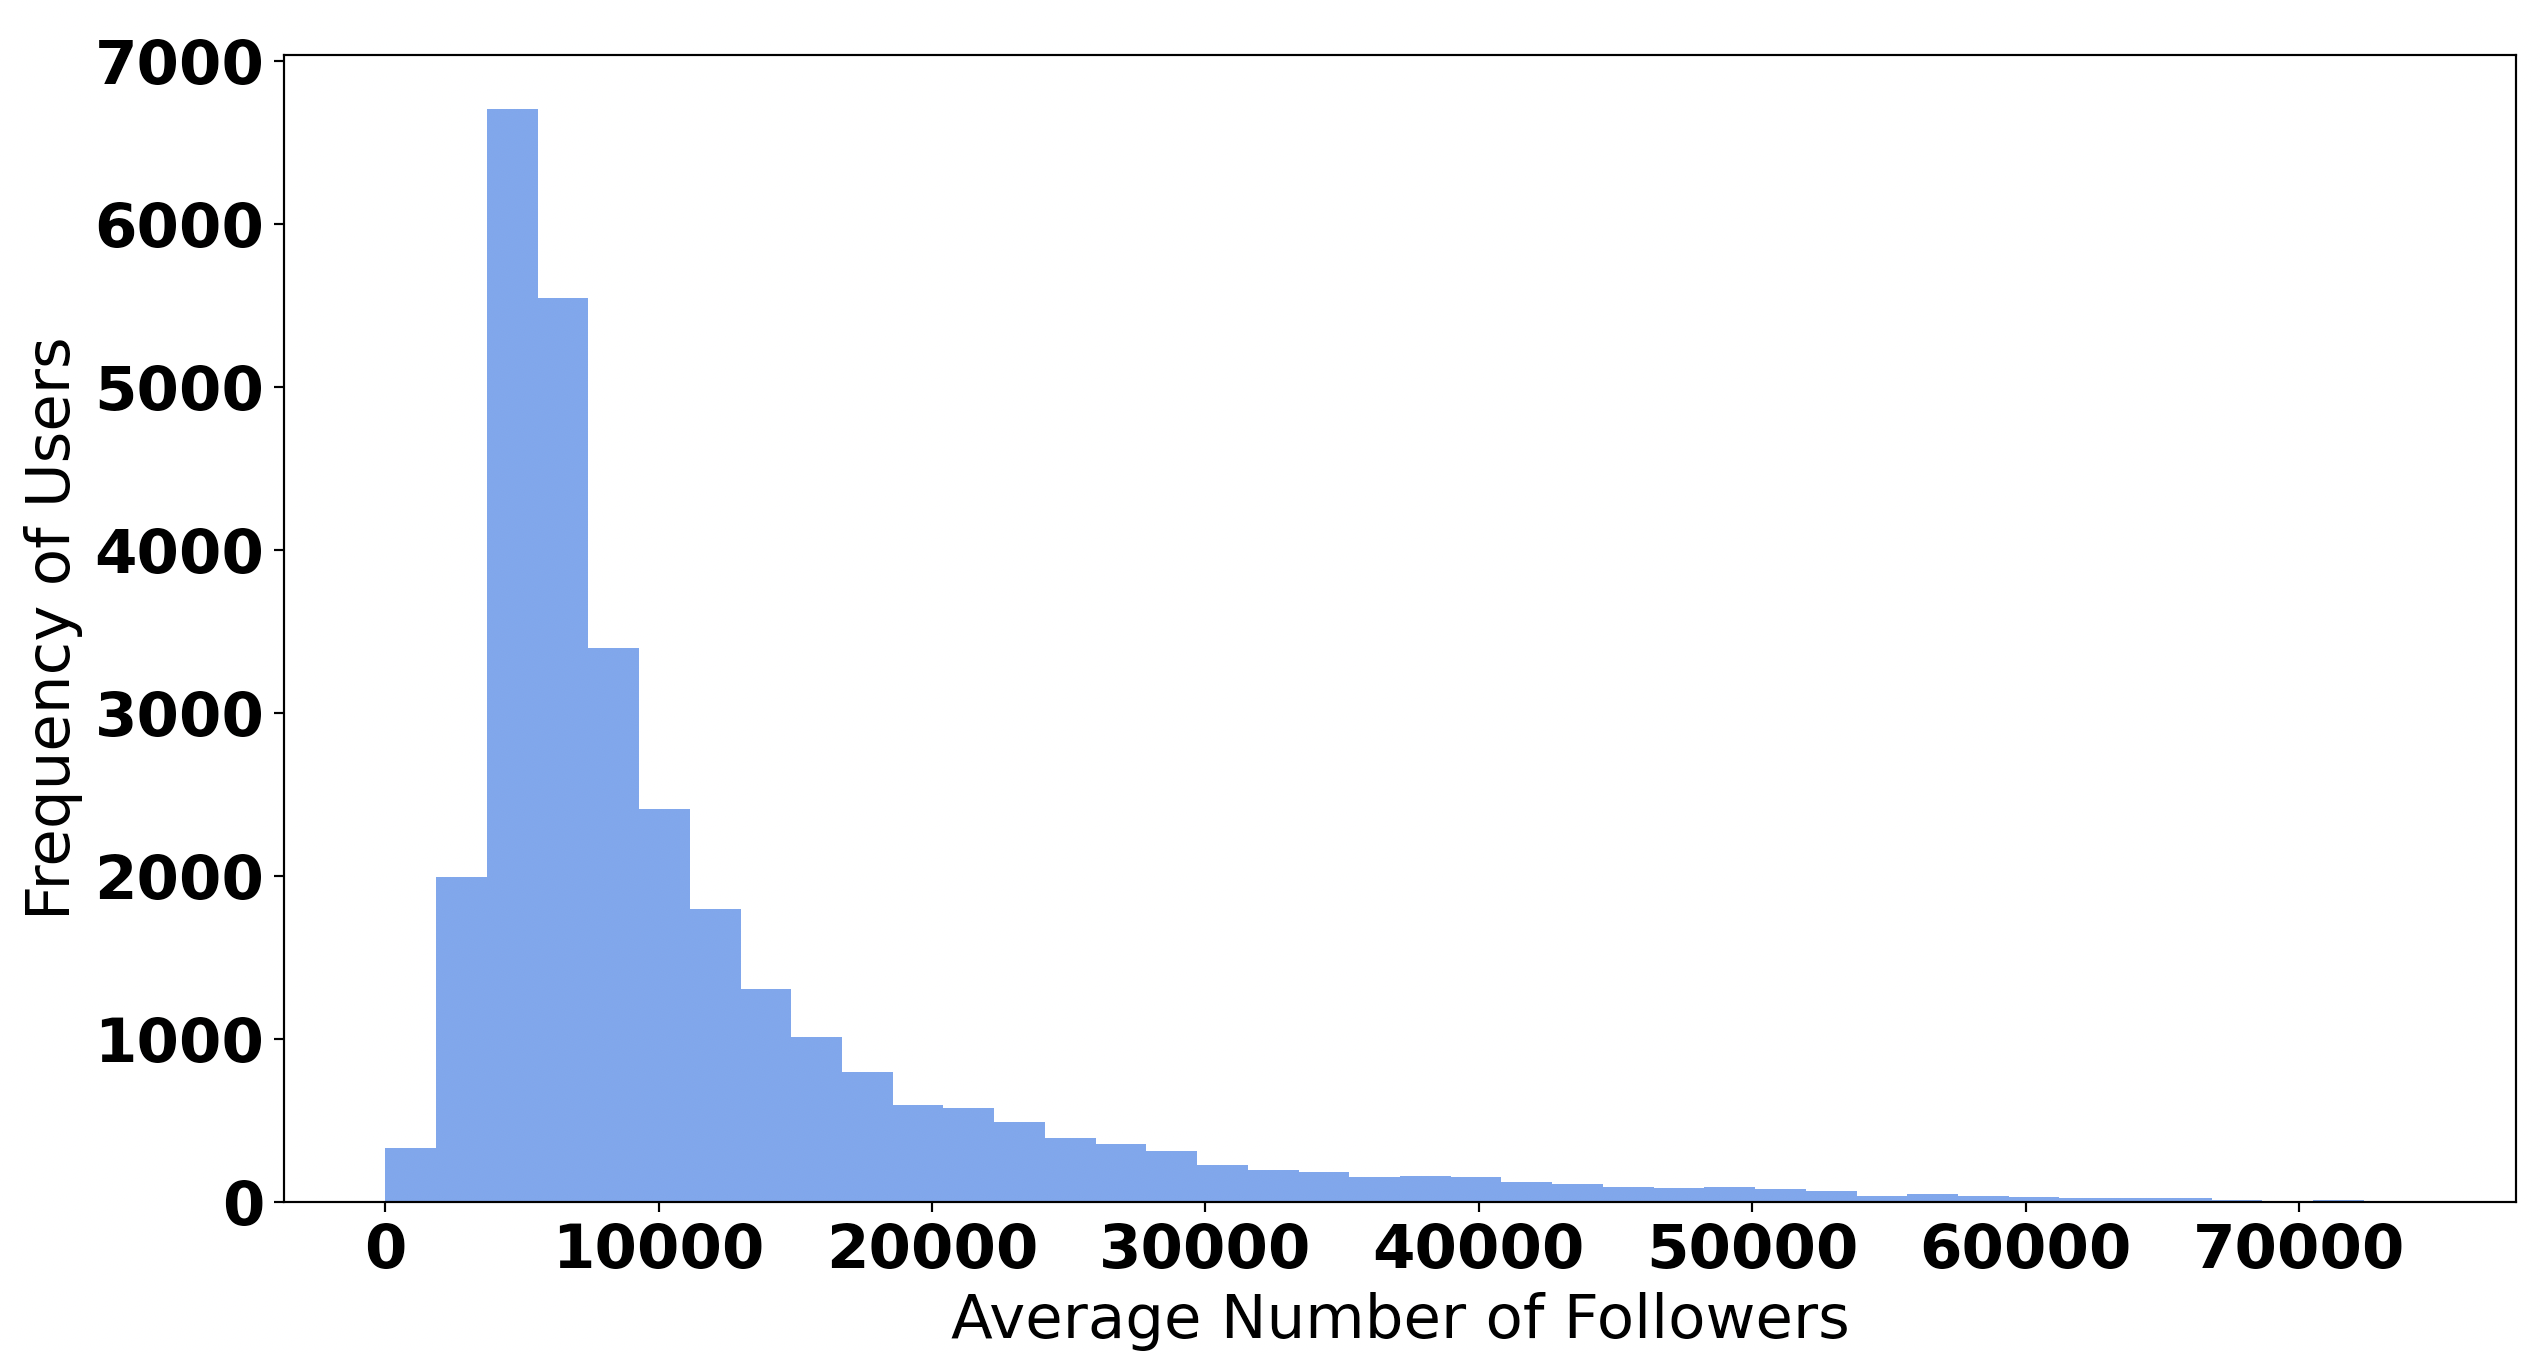
\includegraphics[width=7cm]{p3.png}
\caption{Histogram of User's Average Number of Followers}
\end{figure}

\textbf{Follower count rates.} We begin by analyzing the change in users’ follower numbers as they post more tweets. Our goal is to quantify the impact of a tweet on their number of followers by examining the rate of change of followers. To visualize our analysis, we have included a plot of a single user's time series data of all tweets made, including their most viral tweet, and the number of followers they had at that time (figure 5). For each user will focus our analysis around the date of their viral tweet (red line) and compare the rate of follower gain before and after that point.\\

\begin{figure}[h]
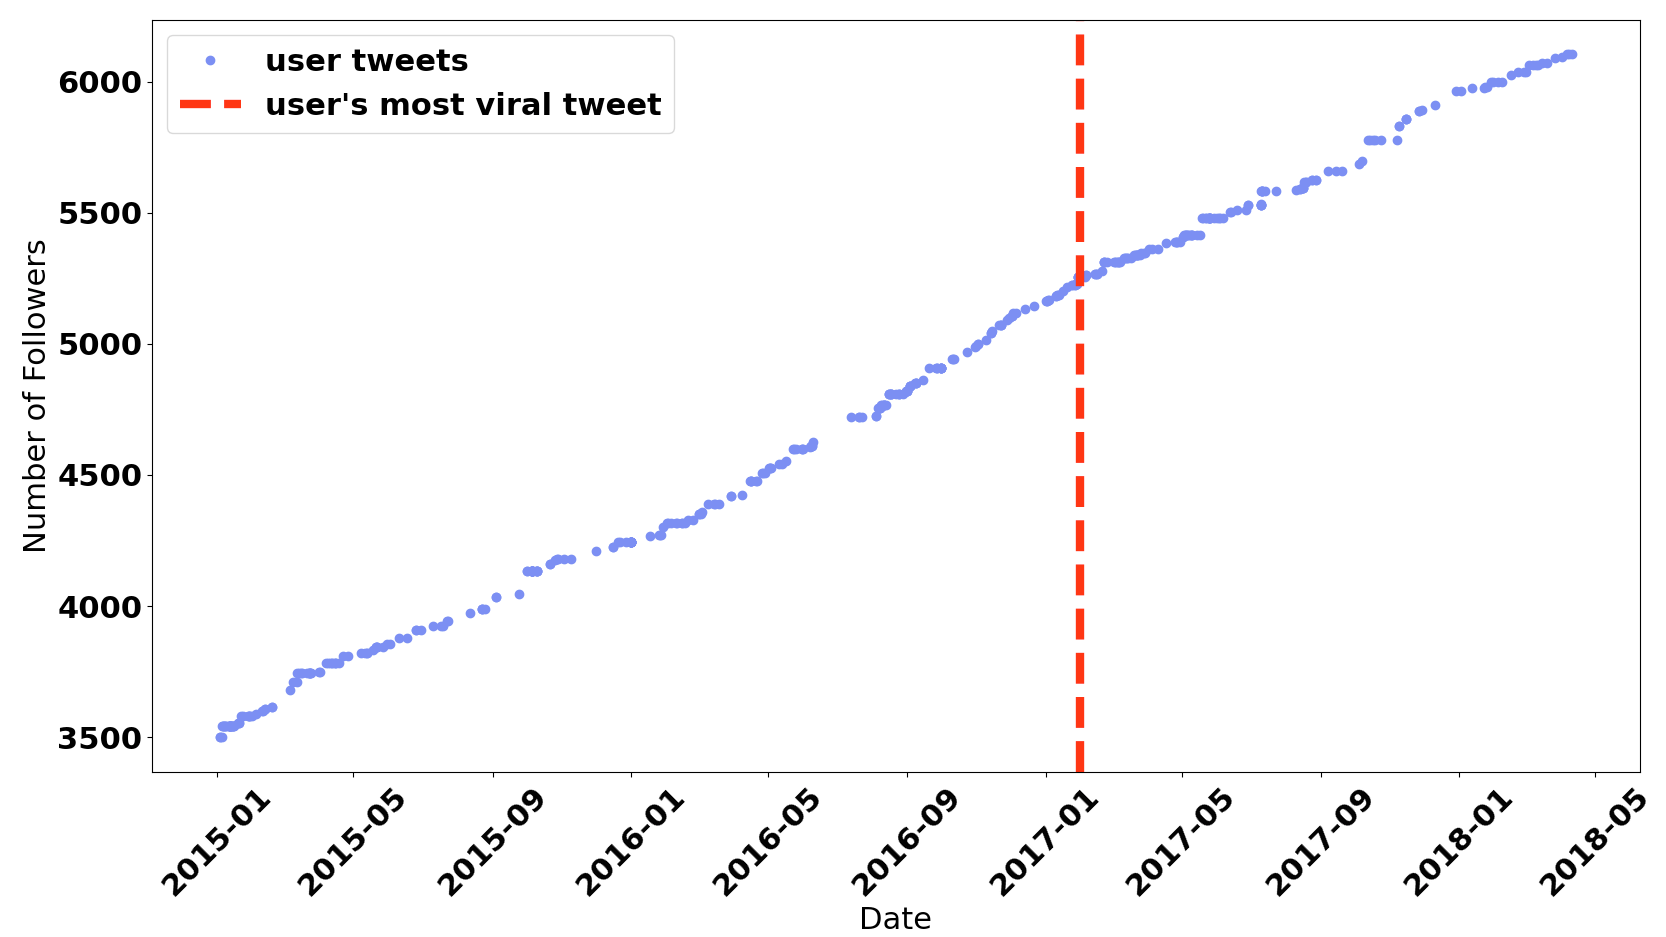
\includegraphics[width=7cm]{p5.png}
\caption{Scatterplot of Number of Followers at Time of Each Tweet for User 10000642}
\end{figure}

For each user, we calculated the difference in number of followers between each tweet. We normalized the resulting values for each user as the rate of change in followers per day by dividing the change in followers by the number of days between the tweets. Users lacking sufficient data to compute these rates were discarded. We found the average change in number of followers per day to be 8.875, indicating that active users generally see their follower counts increase by 8.875 each day.\\

We proceeded to divide the users into buckets based on their follower count at the time of their viral tweet to control for differences due to different scales of following networks. Users were divided into the 9 buckets in Figure 6 based on follower counts.
%%FOLLOWER COUNT TABLE

\begin{figure}[H]
\begin{tabular}{ | m{1cm} | m{3cm} |m{1.5cm} | } 
  \hline
    Bucket & Follower Count & Number of Users \\ 
  \hline
  1 & [0,1000) & 32\\ 
  \hline
  2 & [1000,5000) & 701 \\ 
  \hline
  3 & [5000,10000) & 1640\\ 
  \hline
  4 & [10000,20000) & 1456 \\ 
  \hline
  5 & [20000,30000) & 632 \\ 
  \hline
  6 & [30000,40000)&345 \\ 
  \hline
  7 & [40000,50000) & 206\\ 
  \hline
  8 & [50000,60000) & 141 \\ 
  \hline
  9 & [60000,80000)& 72 \\ 
  \hline
\end{tabular}\\
\caption{Bucket Categories According to Follower Count}
\end{figure}
For each bucket, we computed each user’s mean follower rate per day one week prior, one week after, and one month after their viral tweet. If there were no user entries for any of these time intervals, we discarded the user from our analysis. We compute two differences: 1) the difference between follower rates one week after vs. one week before and 2) the difference between follower rates one month after and one week before. We use the weekly and monthly difference to evaluate the short and long term impact of viral tweets respectively. We chose to look at the median of means before the mean of means because user Twitter career data distributions are heavily tailed, with certain viral tweets receiving high engagement. This gave us a general idea of the follower rate over time for each group of users. We then took the mean of means for each bucket to use for statistical inference.


\section{Results}
Based on the median of the means, we saw numerically that there was a trend for an increase in followers after a viral tweet (Figures 7 and 9). We used statistical inference to quantify this relationship. We performed both a single tailed t-test and a two-tailed t-test to check for a significant difference between follower rates before the tweet and after the tweet.\\

\noindent\textbf{Single-tailed T-test:} For each user bucket, we perform the following test.
\begin{itemize}
\item Null Hypothesis: The mean rate of follower increase is less than or equal to 0.
\item Alternative: The mean rate of follower increase is greater than 0.
\end{itemize}

\noindent\textbf{Two-tailed T-test}: For each user bucket, we perform the following test.
\begin{itemize}
  \item Null Hypothesis: The mean rate of follower increase is 0.
  \item Alternative: The mean rate of follower increase is not 0.
\end{itemize}

Figure 8 and Figure 10  display our resulting t-test scores. Considering the difference in average weekly rates, we see the largest t-statistic with bucket 9 which includes users with 60,000 - 79,999 followers. We plot a histogram of the difference in average follower rates a week before and after users’ viral tweets in Figure 11. We see that the data is somewhat normally distributed, with a heavy tail of larger values.\\

%this table will have info for the week before and week after comparison
\begin{center}
\begin{figure}[H]
\begin{tabular}{ | m{1.5cm} | m{2cm} |m{2cm} | } 
  \hline
    Bucket  & Change in Follower Rate Median of Mean & Change in Follower Rate Mean of Mean \\ 
  \hline
  1 & 1.940 & 23.157  \\ 
  \hline
  2 & 0.267 & 5.226  \\  
  \hline
  3 & 0.000 & 1.614  \\ 
  \hline
  4 & 0.675 & -1.917  \\  
  \hline
  5 & 1.842 & 13.848  \\ 
  \hline
  6 & 1.452 & 3.308  \\  
  \hline
  6 & 4.015 & 10.630  \\  
  \hline
  6 & 6.214 & 18.419  \\  
  \hline
  6 & 3.612 & 12.166 \\  
  \hline
\end{tabular}
\caption{Analysis of Average Change in Follower Rate From Week Before Viral Tweet and Week After}
\end{figure}


%this table will have info for the week before and week after comparison
\begin{figure}[H]
\begin{tabular}{ | m{1.5cm} | m{2cm} |m{2cm} | } 
  \hline
    Bucket  &  Standard Error & T-Statistic\\ 
  \hline
  1 & 72.481 & 0.319  \\ 
  \hline
  2 & 175.083 & 0.030  \\  
  \hline
  3 & 76.853 & 0.021  \\ 
  \hline
  4 & 194.769 & -0.010  \\  
  \hline
  5 & 120.405 & 0.115  \\ 
  \hline
  6 & 56.887 & 0.058  \\  
  \hline
  7 & 67.178 & 0.158  \\ 
  \hline
  8 & 99.539 & 0.185  \\  
  \hline
  9 & 30.096 & 0.404  \\  
  \hline
\end{tabular}
\caption{Statistical Inference on Mean of Means For Week Before Viral Tweet and Week After}
\end{figure}


%this table will have info for the week before and month after comparison
\begin{figure}[H]
\begin{tabular}{ | m{1.5cm} | m{2cm} |m{2cm} | } 
  \hline
    Bucket  & Change in Follower Rate Median of Mean & Change in Follower Rate Mean of Mean \\ 
  \hline
  1 & 2.936 & 14.727  \\ 
  \hline
  2 & 0.548 & -5.408  \\  
  \hline
  3 & 0.353 & -4.878  \\ 
  \hline
  4 & 0.596 & -9.518  \\  
  \hline
  5 & 0.749 & 0.0317  \\ 
  \hline
  6 & 0.1780 & -6.240  \\  
  \hline
  7 & 1.564 & 0.547  \\ 
  \hline
  8 & 1.467 & 4.141  \\  
  \hline
  9 & 3.111 & 4.851  \\  
  \hline
\end{tabular}
\caption{Analysis of Average Change in Follower Rate From Week Before Viral Tweet and Month After}
\end{figure}

%this table will have info for the week before and month after comparison
\begin{figure}[H]
\begin{tabular}{ | m{1.5cm} | m{2cm} |m{2cm} | } 
  \hline
    Bucket  &  Standard Error & T-Statistic\\ 
  \hline
  1 & 45.155 & 0.326  \\ 
  \hline
  2 & 149.917 & -0.036  \\  
  \hline
  3 & 43.440 & -0.112  \\ 
  \hline
  4 & 189.472 & -0.050  \\  
  \hline
  5 & 45.304 & 0.001  \\ 
  \hline
  6 & 51.837 & -0.120  \\  
  \hline
  7 & 58.929 & 0.009 \\ 
  \hline
  8 & 66.045 & 0.063  \\  
  \hline
  9 & 22.708 & 0.214  \\  
  \hline
\end{tabular}
\caption{Statistical Inference on Mean of Means For Week Before Viral Tweet and Month After}
\end{figure}
\end{center}

\begin{figure}[h]
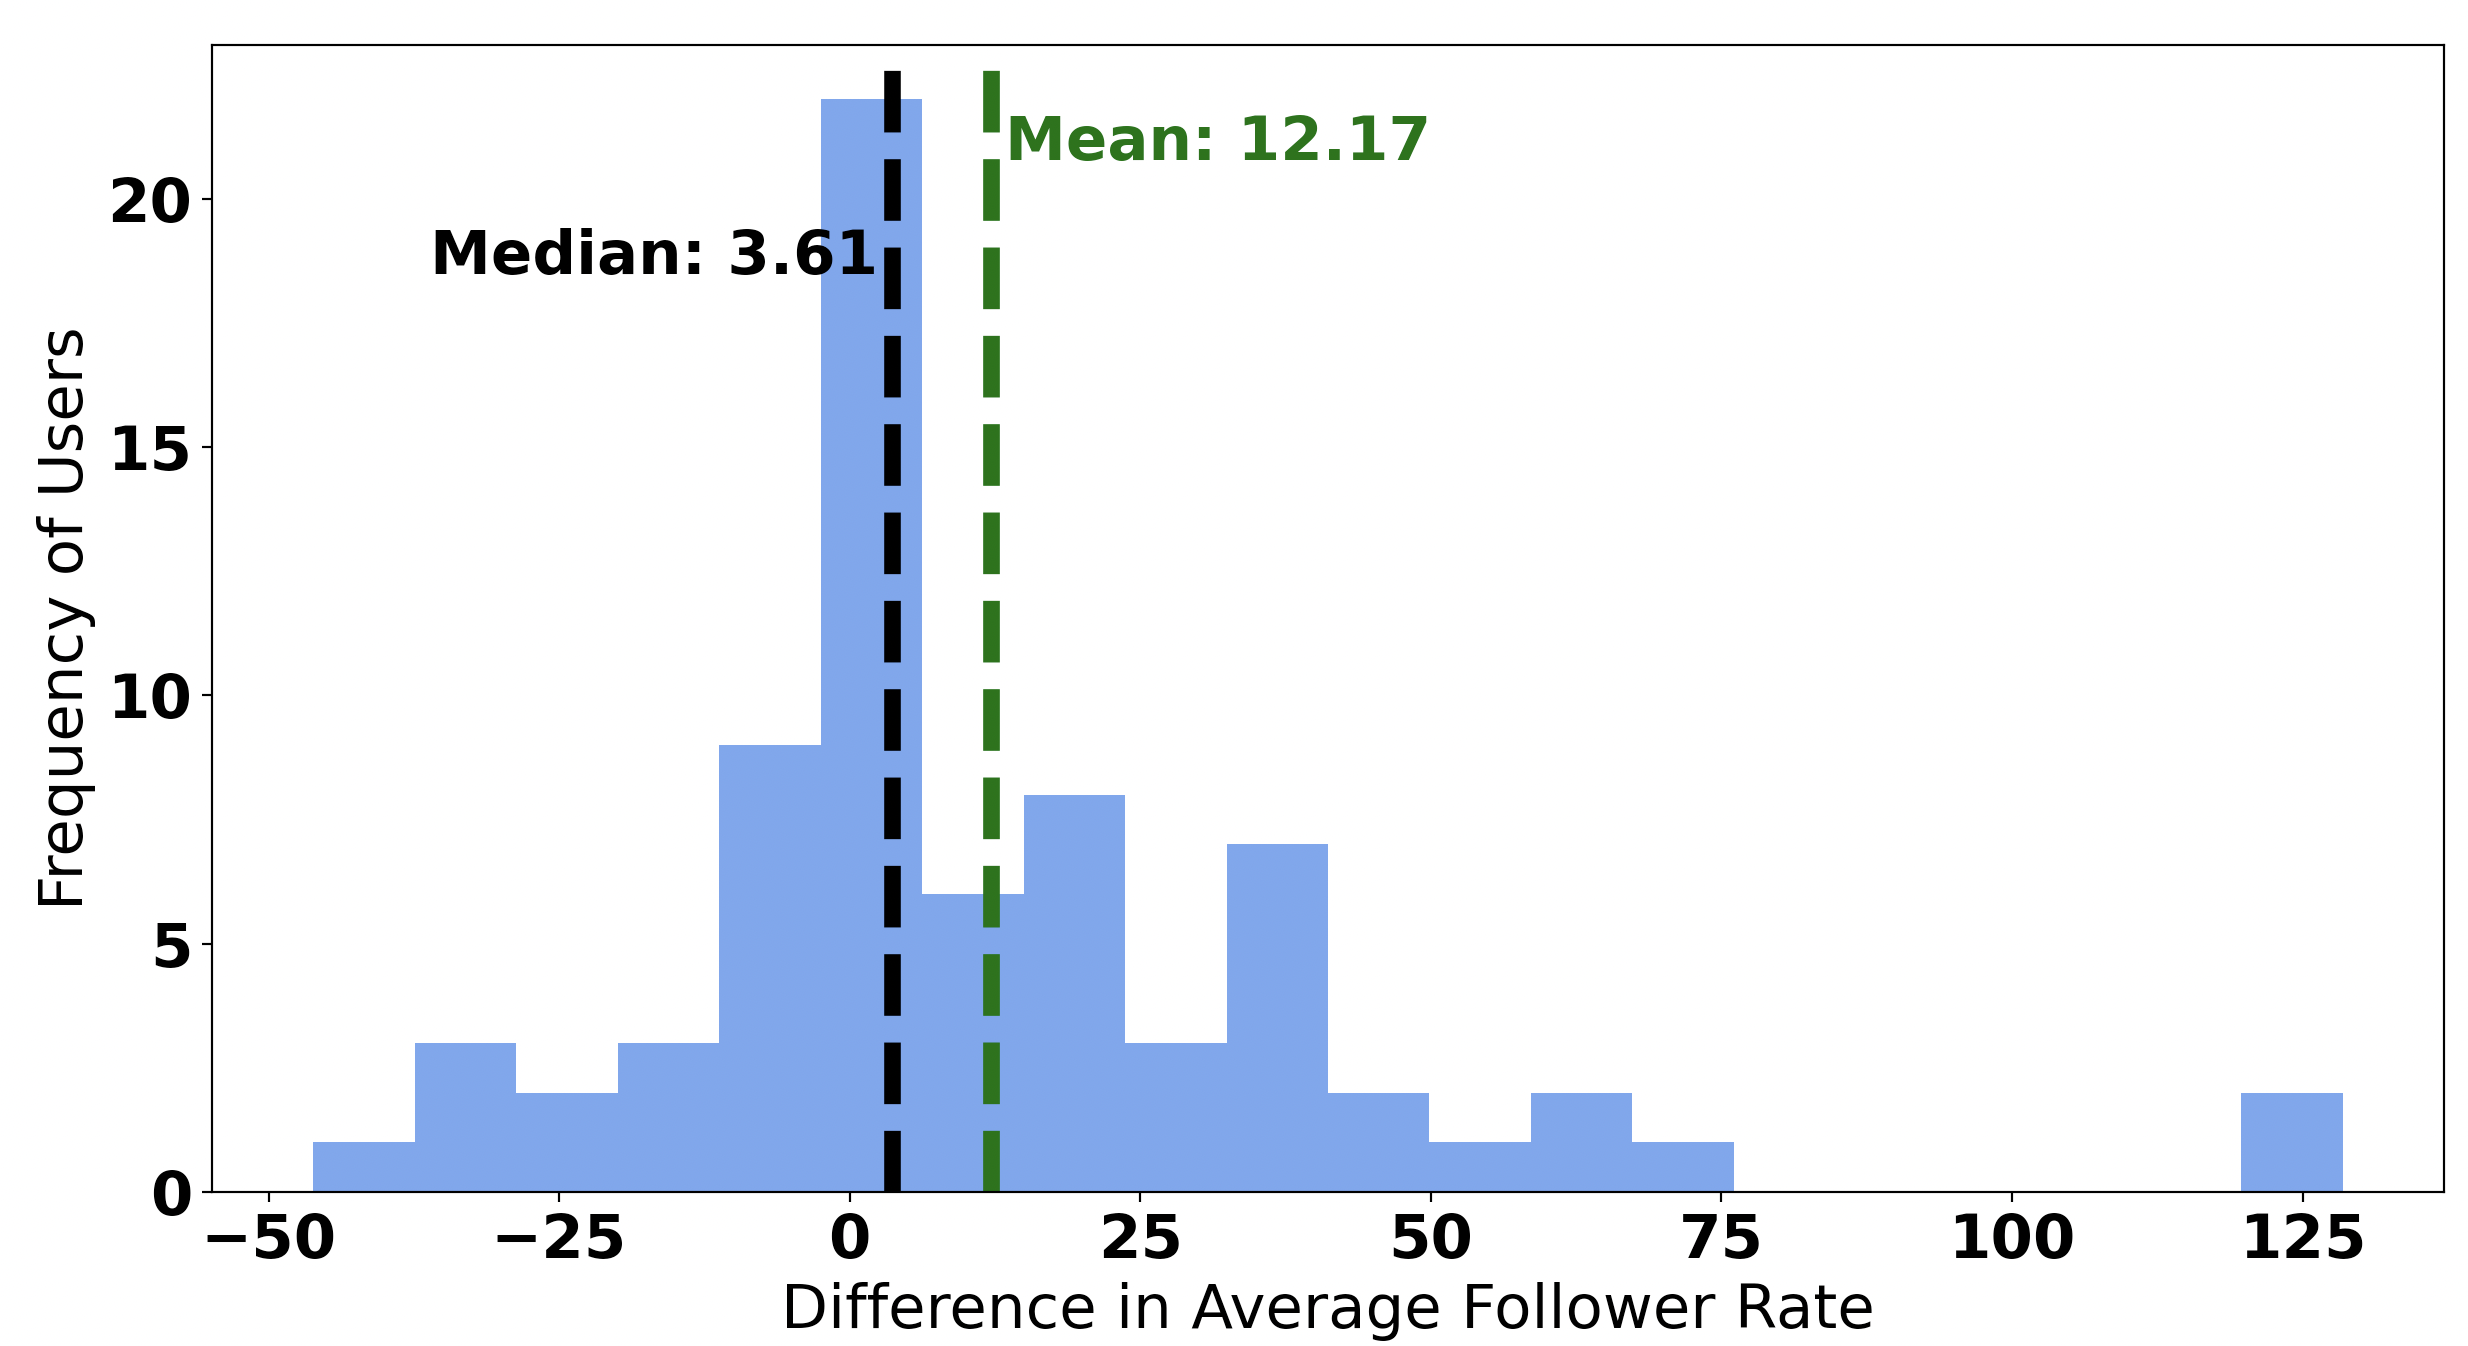
\includegraphics[width=7cm]{p4.png}
\caption{Histogram of the Weekly Difference in \\Average Follower Rates for Bucket 9}
\end{figure}

Given that none of our resulting t-test scores had a large enough absolute value, we fail to reject the null hypothesis with a p-value = .05 threshold for both the single-tailed and two-tailed analysis. Therefore, we are unable to assert that this relationship is one of statistical significance at this time.\\


\section{Conclusion and Future Work}

Learning that our method described in this study did not produce significant results about the relationship between follower count and rate of increase of followers after a user's most viral tweet helps to point us in a new direction for our future work. This brings into question what other variables could be contributing to the change in follower rates. \\

Our selected dataset was one of few with time series related data with complete lifetime user information. Unfortunately, many of the follower counts were estimated using crawls from the Wayback Machine. Ideally, data used could be official follower and retweet data pulled from the Twitter API at a recurring interval. We split users into buckets based on follower count because we intuitively understand that the rate of increase of followers is likely going to be larger for a user that already has a higher following count. However, we acknowledge that the relationship between what that following count is and how the number contributes to the rate of increase is not fully explored. Furthermore, we use the change in followers per day a week before viral tweets as the baseline measurement for a user's normal rate of growth. This may be an inaccurate metric because we are not accounting for their potential traction leading up to their most viral tweet.\\


There are also opportunities to use other statistical methods to evaluate the significance of the change in follower rates before and after viral tweets. We used t-tests to evaluate whether or not the changes were statistically significant, but needed to make a large assumption that the data was approximately normally distributed. In the future, we can look into relaxing this normal distribution assumption and using other methods that do not rely on this assumption, such as Bayesian statistical inferences.

\section{Acknowledgements}
We would like to offer our special thanks to Dr. Ymir Vigfusson from the Emory Computer Science department for assisting us with our data analysis. His willingness to give his time and advice is greatly appreciated. We would also like to thank Garimella and West for their data collection and for making this dataset public. We would not have been able to complete our analysis without it. 

\section{Data and Code}
We have created a Google Drive folder containing our dataset and code used for this paper. You can find the folder here: shorturl.at/ksCZ6 \\
%----------------------------------------------------------------------------------------
%	REFERENCE LIST
%----------------------------------------------------------------------------------------
\pagebreak
% \bibliography{cs385} 
% \bibliographystyle{ieeetr}
\printbibliography

% \nocite{*}
% \bibliographystyle{unsrt}
% \bibliography{ref}

% \begin{thebibliography}{99} % Bibliography - this is intentionally simple in this template

% %#####  PUT REFERENCES HERE (you need at least one regrading a famous exploit ###### 
% %##### Remove this example before you hand in !!! ######## 



% \bibitem[1]{}
% {\em Twitter: most users by country.} (2021, November 19). Statista. https://www.statista.com/statistics/242606/number-of-active-twitter-users-in-selected-countries/
% % \newblock Assortative pairing and life history strategy - a cross-cultural study.
% % \newblock {\em Human Nature}, 20:317--330.
 

% \end{thebibliography}
%----------------------------------------------------------------------------------------

%----------------------------------------------------------------------------------------
% REFERENCE LIST
%----------------------------------------------------------------------------------------

% @Inbook{CSPP,
% author={Bryant, Randal E. 
% and O'Hallaron, David R.},
% TITLE={Computer Systems},
% SUBTITLE={A Programmer's Perspective},
% YEAR={2016},
% PUBLISHER={Pearson Education Limited},
% EDITON={Third},
% PAGES={875--911},
% }

% \section{Appendix A}
% {\color{blue} \emph  
% Here you would put extra material or very detailed descriptions etc. etc. 
% If you have a lot of extra material you could even have more appendix sections. 
% }
%----------------------------------------------------------------------------------------

\end{document}